\documentclass[runningheads]{llncs}

\usepackage[T1]{fontenc}
\usepackage[utf8]{inputenc}
\usepackage{graphicx}
\usepackage{amsmath,amssymb}
\usepackage{booktabs}
\usepackage{multirow}
\usepackage{algorithm}
\usepackage{algpseudocode}
\usepackage{url}


\begin{document}

\title{Evaluating Monolingual and Multilingual Training in English–Hindi Speech Emotion Recognition Using MFCC-Based Recurrent Neural Networks}

\titlerunning{Monolingual and Multilingual SER Using MFCC-Based RNNs}

\author{
Sudipta Bhattacharya\inst{1} \and
Sandipan Sahu\inst{2} \and
Rivu Panda\inst{1} \and
Nayan Bhudolia\inst{1} \and
Anik Chiney\inst{1}$^{*}$ \and
Farhan Wajid\inst{1}
}

\authorrunning{S. Bhattacharya et al.}

\institute{
Institute of Engineering \& Management,\\
School of University of Engineering \& Management,\\
Kolkata, West Bengal, India\\
\email{\{bhattacharya.sudipta, pandarivu2004, nayan.bhudolia, anikchiney130$^{*}{Corresponding author}$, farhanwajid05\}@gmail.com}
\and
Department of Computer Science and Engineering,\\
Amity University, Kolkata, India\\
\email{sahusandipan@gmail.com}
}

\maketitle

\begin{abstract}
Speech Emotion Recognition (SER) is identifying emotional states from speech signals. SER plays a vital role in enhancing human–computer interaction (HCI). Maximum of the existing studies focus on monolingual settings, i.e. model has been trained on a specific language dataset. Performance of the monolingual model often degrades when exposed to speech from different languages. This proposed study presents a controlled bilingual evaluation of monolingual and multilingual training protocols for SER. In this study English (RAVDESS) and Hindi (IESC) datasets have been used. This study considers Mel-Frequency Cepstral Coefficients (MFCC) as acoustic features and systematically uses recurrent architectures including Long Short-Term Memory (LSTM) and Bidirectional LSTM (Bi-LSTM) as the benchmarked models. Experiment has been conducted under monolingual (EN→EN, HI→HI) and multilingual pooling (EN→EN/HI) settings using stratified cross-validation. Experimental results show that Bi-LSTM model consistently outperforms the unidirectional LSTM model. The Bi-LSTM model is more capable of capturing contextual dependencies in both temporal directions. Multilingual training improves the robustness of the model and reduces performance variance across folds. However, partial degradation still occurs due to cross-language variability. Findings of this study highlight the effectiveness of lightweight MFCC-based recurrent baselines for bilingual low-resource SER, at the same time also identifying the limitations that motivate future extensions of using domain-robust and attention-based models.
\keywords{Speech Emotion Recognition (SER) \and Deep Learning \and MFCC \and LSTM \and Bi-LSTM \and Multilingual Learning }
\end{abstract}

\section{Introduction}

Emotion is a fundamental component of human communication, inherently conveyed through variations in speech attributes such as pitch, energy, rhythm etc. People show emotion through pitch, loudness, speed, and pauses. Speech Emotion Recognition (SER) aims to automatically detect these emotional states from audio signals. It can make human–computer talks more natural and helpful \cite{ElAyadi2011Survey,Schuller2011Challenge}. SER contribute significantly to applications like intelligent virtual assistants, affect-aware systems, and psychological support tools. SER is useful in call centres to track customer mood. It can also help smart assistants react in a better way. In the future, SER can support learning apps and health support systems that watch stress or sadness, but it should not be used as a medical test \cite{Schuller2011Challenge,Bhattacharya2024CrossLingual}.

Traditional SER uses classical machine learning (ML) models and generally rely on handcrafted features. Classical ML models often face challenges in generalization across multiple datasets and languages. Previous SER systems often used hand-made features and classic models. These systems depend a lot on the selected features. They may fail when the speaker, mic, or room changes. Accuracy also drops when the language changes. Many of them need careful tuning for each dataset \cite{ElAyadi2011Survey}.

Introduction of DL models reduces the need for manual feature design. Recurrent models like LSTM can learn time patterns in speech  \cite{Hochreiter1997LSTM}. Bi-LSTM model is capable to use both past and future context in the signal. Bi-directional information improves the performance of emotional pattern recognition  \cite{Graves2005BiLSTM}. The most significant factor in SER is scarcity of proper datasets of many local languages. Many of the local and low-resource languages don’t have significant amount of speech emotion datasets. Sometimes data may exist, but the labels are limited or improper. Publicly available datasets like RAVDESS are widely used for English SER work  \cite{Livingstone2018RAVDESS}. Datasets like IEMOCAP are also common in research and allow strong model testing  \cite{Busso2008IEMOCAP}. These datasets are useful, but they do not cover all languages and speaking styles.

Despite significant work done, still SER systems face practical challenges due to language barriers, cultural differences, and dataset limitations. Most existing research focuses on monolingual datasets, limiting model applicability in multilingual real-world scenarios. This study addresses this gap by conducting a comparative analysis of LSTM, and Bi-LSTM architectures using MFCC-based features across multiple emotional speech datasets--RAVDESS (English) and IESC (Hindi). Evaluations under monolingual, cross-lingual, and multilingual settings assess model generalization and robustness, highlighting the strengths and limitations of current approaches.

This paper studies SER across English and Hindi. We compare LSTM and Bi-LSTM using MFCC features, which are still widely used in SER baselines \cite{Eyben2010OpenSMILE,Bhattacharya2024MultimodalKFold}. We also test a self-supervised model approach using WavLM. Self-supervised speech models learn useful speech patterns from large audio data without emotion labels \cite{Baevski2020Wav2Vec2,Chen2022WavLM,Hsu2021HuBERT,bhattacharya2022deep}. We check performance in monolingual, and multilingual settings. This helps us see what works well when language changes, and what still fails. Here, the contribution of our proposed work has been stated in the following:
\begin{itemize}
    \item We have proposed a SER baseline for English and Hindi using MFCC with LSTM and Bi-LSTM.
    \item Extensively tested the models in monolingual, multilingual settings.
\end{itemize}

The remainder of the paper is organized as follows.  Section II reviews related work. Section III explains the datasets, features, and models. Section IV presents results and analysis and section V discussion. Section VI concludes the paper and lists future work.

\section{Literature Review}
There have been various research articles on emotion recognition through human-computer interaction. In this section, we review past work on speech emotion recognition. We focus on four main points. First, many studies use MFCC or log-mel features as strong baselines. Second, deep models like CNN, LSTM, and BiLSTM often beat classic models because they learn time patterns. Third, results drop when training and testing languages or datasets differ, so cross-lingual SER is still hard. Fourth, self-supervised speech models can improve transfer across datasets because they learn general speech patterns from large audio data.

Table~\ref{tab:related} presents a summary of different SER studies. which include MFCC features, and different architectures like CNN, recurrent models, CNN-RNN architectures, attention-based architecture and transfer learning with multilingual models. Mose of the Prior work consistently shows that MFCC remains a strong low-compute audio feature, while deep sequence models (LSTM/Bi-LSTM) and attention mechanisms improve temporal modeling. However, most of the works are dataset and language dependent. Performance of these models degrades when exposed under different language or works in a low-resource conditions. Motivating from these research gaps and propose benchmarks MFCC+LSTM/Bi-LSTM on English (RAVDESS) and Hindi (IESC) under mono-lingual and multi-lingual training protocols to quantify generalization across languages.

\begin{table}[!htbp]
\caption{Summary of representative related works.}
\label{tab:related}
\centering
\renewcommand{\arraystretch}{1.15}
\begin{tabular}{p{2cm} p{2.8cm} p{3.2cm} p{2.2cm} p{5cm}}
\toprule
\textbf{Author(s)} & \textbf{Model / Technique} & \textbf{Feature Representation} & \textbf{Dataset / Language} & \textbf{Key Contributions / Findings} \\
\midrule

Bhagath et al. ~\cite{Bhagath2026MultilingualCNN} 
& CNN-based model 
& MFCC 
& Hindi, Telugu, Indian accented English 
& Addressed low-resource multilingual spoken language modeling. Tested different input combinations. Reported highest accuracy for Telugu (99.1\%). \\

\midrule

Yadav et al. ~\cite{Yadav2026Misogyny} 
& Transformer-based misogyny detection (XLM-R, mBERT). Multimodal: mBERT + EfficientNet / ResNet. Explainability via SHAP and LIME. 
& Transformer embeddings (text); image features + text features (multimodal); SHAP/LIME attribution outputs. 
& Code-mixed Hindi–English (Hinglish) 
& Proposed an explainable multimodal system and web application. Focused on low-resource and code-mixed settings. Included human evaluation (CUQ, UEQ) and usability analysis. \\

\midrule
Haidar et al. ~\cite{Haidar2025SERLSTM} 
& LSTM neural network 
& MFCC 
& CREMA-D, RAVDESS 
& Used LSTM for temporal modeling of speech emotion. Reported competitive accuracy on small SER datasets. \\

\midrule

Xu et al. ~\cite{Xu2021HeadFusion} 
& Attention-based CNN (ACNN) with Head Fusion (multi-head attention) 
& MFCC 
& IEMOCAP, RAVDESS 
& Proposed Head Fusion to improve robustness. Reported WA and UA $\approx$ 76\% on IEMOCAP. Evaluated noise robustness. \\

\midrule

Li et al. ~\cite{Li2026AAMICASA} 
& Multi-attention CNN: AAM (augmentation) + ICASA (attention refinement) 
& Mel Frequency Cepstral Coefficient (MFCC) features
(39-dimensional: 13 static coefficients plus first- and
second-order derivatives) 
& IEMOCAP, RAVDESS 
& Improved SER via adaptive augmentation and attention refinement. Reported statistically significant accuracy gains. \\

\midrule

Trigeorgis et al. ~\cite{Trigeorgis2016Adieu} 
& End-to-end CNN + RNN 
& Raw waveform input 
& RECOLA (French) 
& Learned emotion directly from raw audio. Outperformed feature-based baselines for continuous emotion prediction. \\

\bottomrule
\end{tabular}
\end{table}

\section{Methodology}

\subsection{Experimental Design}

This study has presented a controlled environment for bilingual SER evaluation under monolingual and multilingual training protocols. In the monolingual configuration, training and testing were performed in the same language dataset (EN→EN and HI→HI). In the multilingual configuration, English and Hindi datasets were combined during training (EN $\cup$ HI), while evaluation was conducted separately on each language. Feature extraction and model architectures were kept identical across all settings to ensure that performance differences arise solely from training configuration.

\subsection{Datasets and Emotion Mapping}

Experiments were conducted using the RAVDESS (English) and Indian Emotional Speech Corpus (IESC, Hindi) datasets. To enable cross-language evaluation, emotion labels were harmonized into a unified five-class space: \textit{Angry, Sad, Happy, Fear}, and \textit{Neutral}. Both datasets consist of acted speech recorded under controlled conditions, ensuring acoustic clarity while potentially limiting real-world generalization.

\subsection{Preprocessing and Augmentation}

All audio samples were converted to mono, resampled to 16 kHz, and standardized to a fixed duration of 3 seconds (48,000 samples). Shorter clips were zero-padded, and longer clips were truncated. To improve robustness, light augmentation including noise injection, time shifting, pitch variation, and time stretching was applied during training. Class imbalance was mitigated using SMOTE applied to feature representations prior to model optimization.

\subsection{Feature Extraction}

Mel-Frequency Cepstral Coefficients (MFCC) were extracted using a 25 ms window and 10 ms hop length. Forty coefficients were computed per frame and padded or truncated to 174 frames, resulting in an input representation of dimension $(174 \times 40)$. MFCC features were selected due to their strong empirical validation in SER literature and computational efficiency, making them appropriate for low-resource bilingual benchmarking.

\subsection{Model Architectures}

Two recurrent architectures were evaluated. The LSTM model consists of two stacked layers (128 and 64 units), followed by dropout regularization (0.3), a dense layer with ReLU activation, and a Softmax output layer. The Bidirectional LSTM (Bi-LSTM) uses the same configuration but processes sequences in both temporal directions, enabling enhanced contextual modeling. Models were trained using RMSprop with categorical cross-entropy loss for 50 epochs and a batch size of 32. Fig. \ref{fig:7} illustrates the complete pipeline of the proposed system, including preprocessing, MFCC feature extraction, and model training using LSTM and Bi-LSTM architectures for monolingual and multilingual. Fig. \ref{fig:proposed_framework} explains that the system takes raw audio input then extracts MFCC features, and processes them using forward and backward LSTM layers. The outputs are combined and passed through a dense layer followed by a softmax activation function to classify emotions such as anger, happiness, sadness, and neutrality.

\subsection{Evaluation Protocol}

Fig. \ref{fig:3} presents the evaluation strategies adopted in this study. In the monolingual setting, models are trained and tested on the same language dataset. But the multilingual setting adds English and Hindi datasets during training while evaluating performance separately on both languages. Data were split using an 80/20 train–test partition. To ensure stable performance estimation, 5-fold stratified cross-validation was applied to the training set while preserving class distribution. Performance was measured using accuracy, precision, recall, and F1-score, reported as mean $\pm$ standard deviation across folds.



\begin{figure}[t]
\centering

\begin{minipage}{0.48\textwidth}
\centering
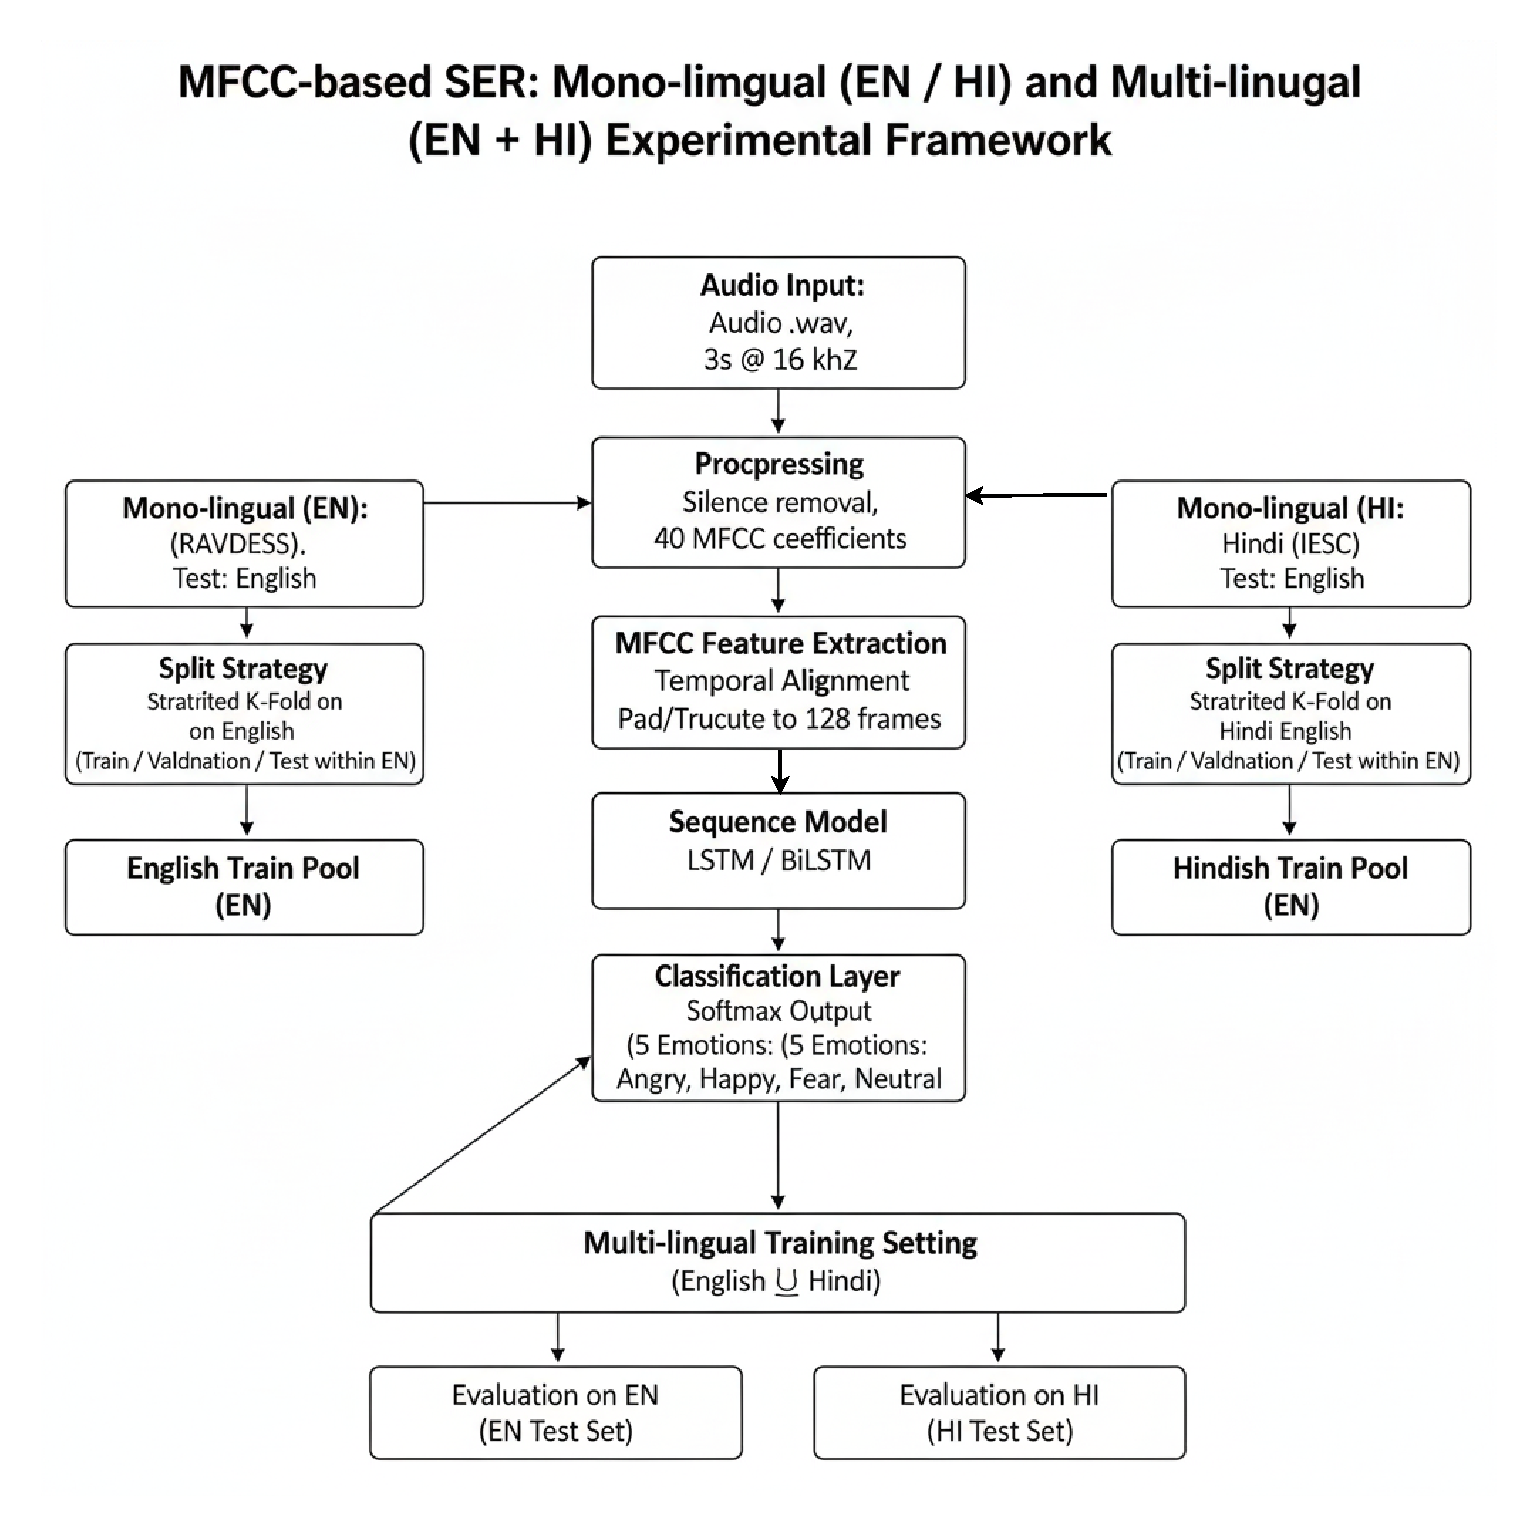
\includegraphics[width=\linewidth]
{images/figure_7.pdf}
\caption{Mono-lingual and Multi-lingual Experimental Framework}
\label{fig:7}
\end{minipage}
\hfill
\begin{minipage}{0.48\textwidth}
\centering
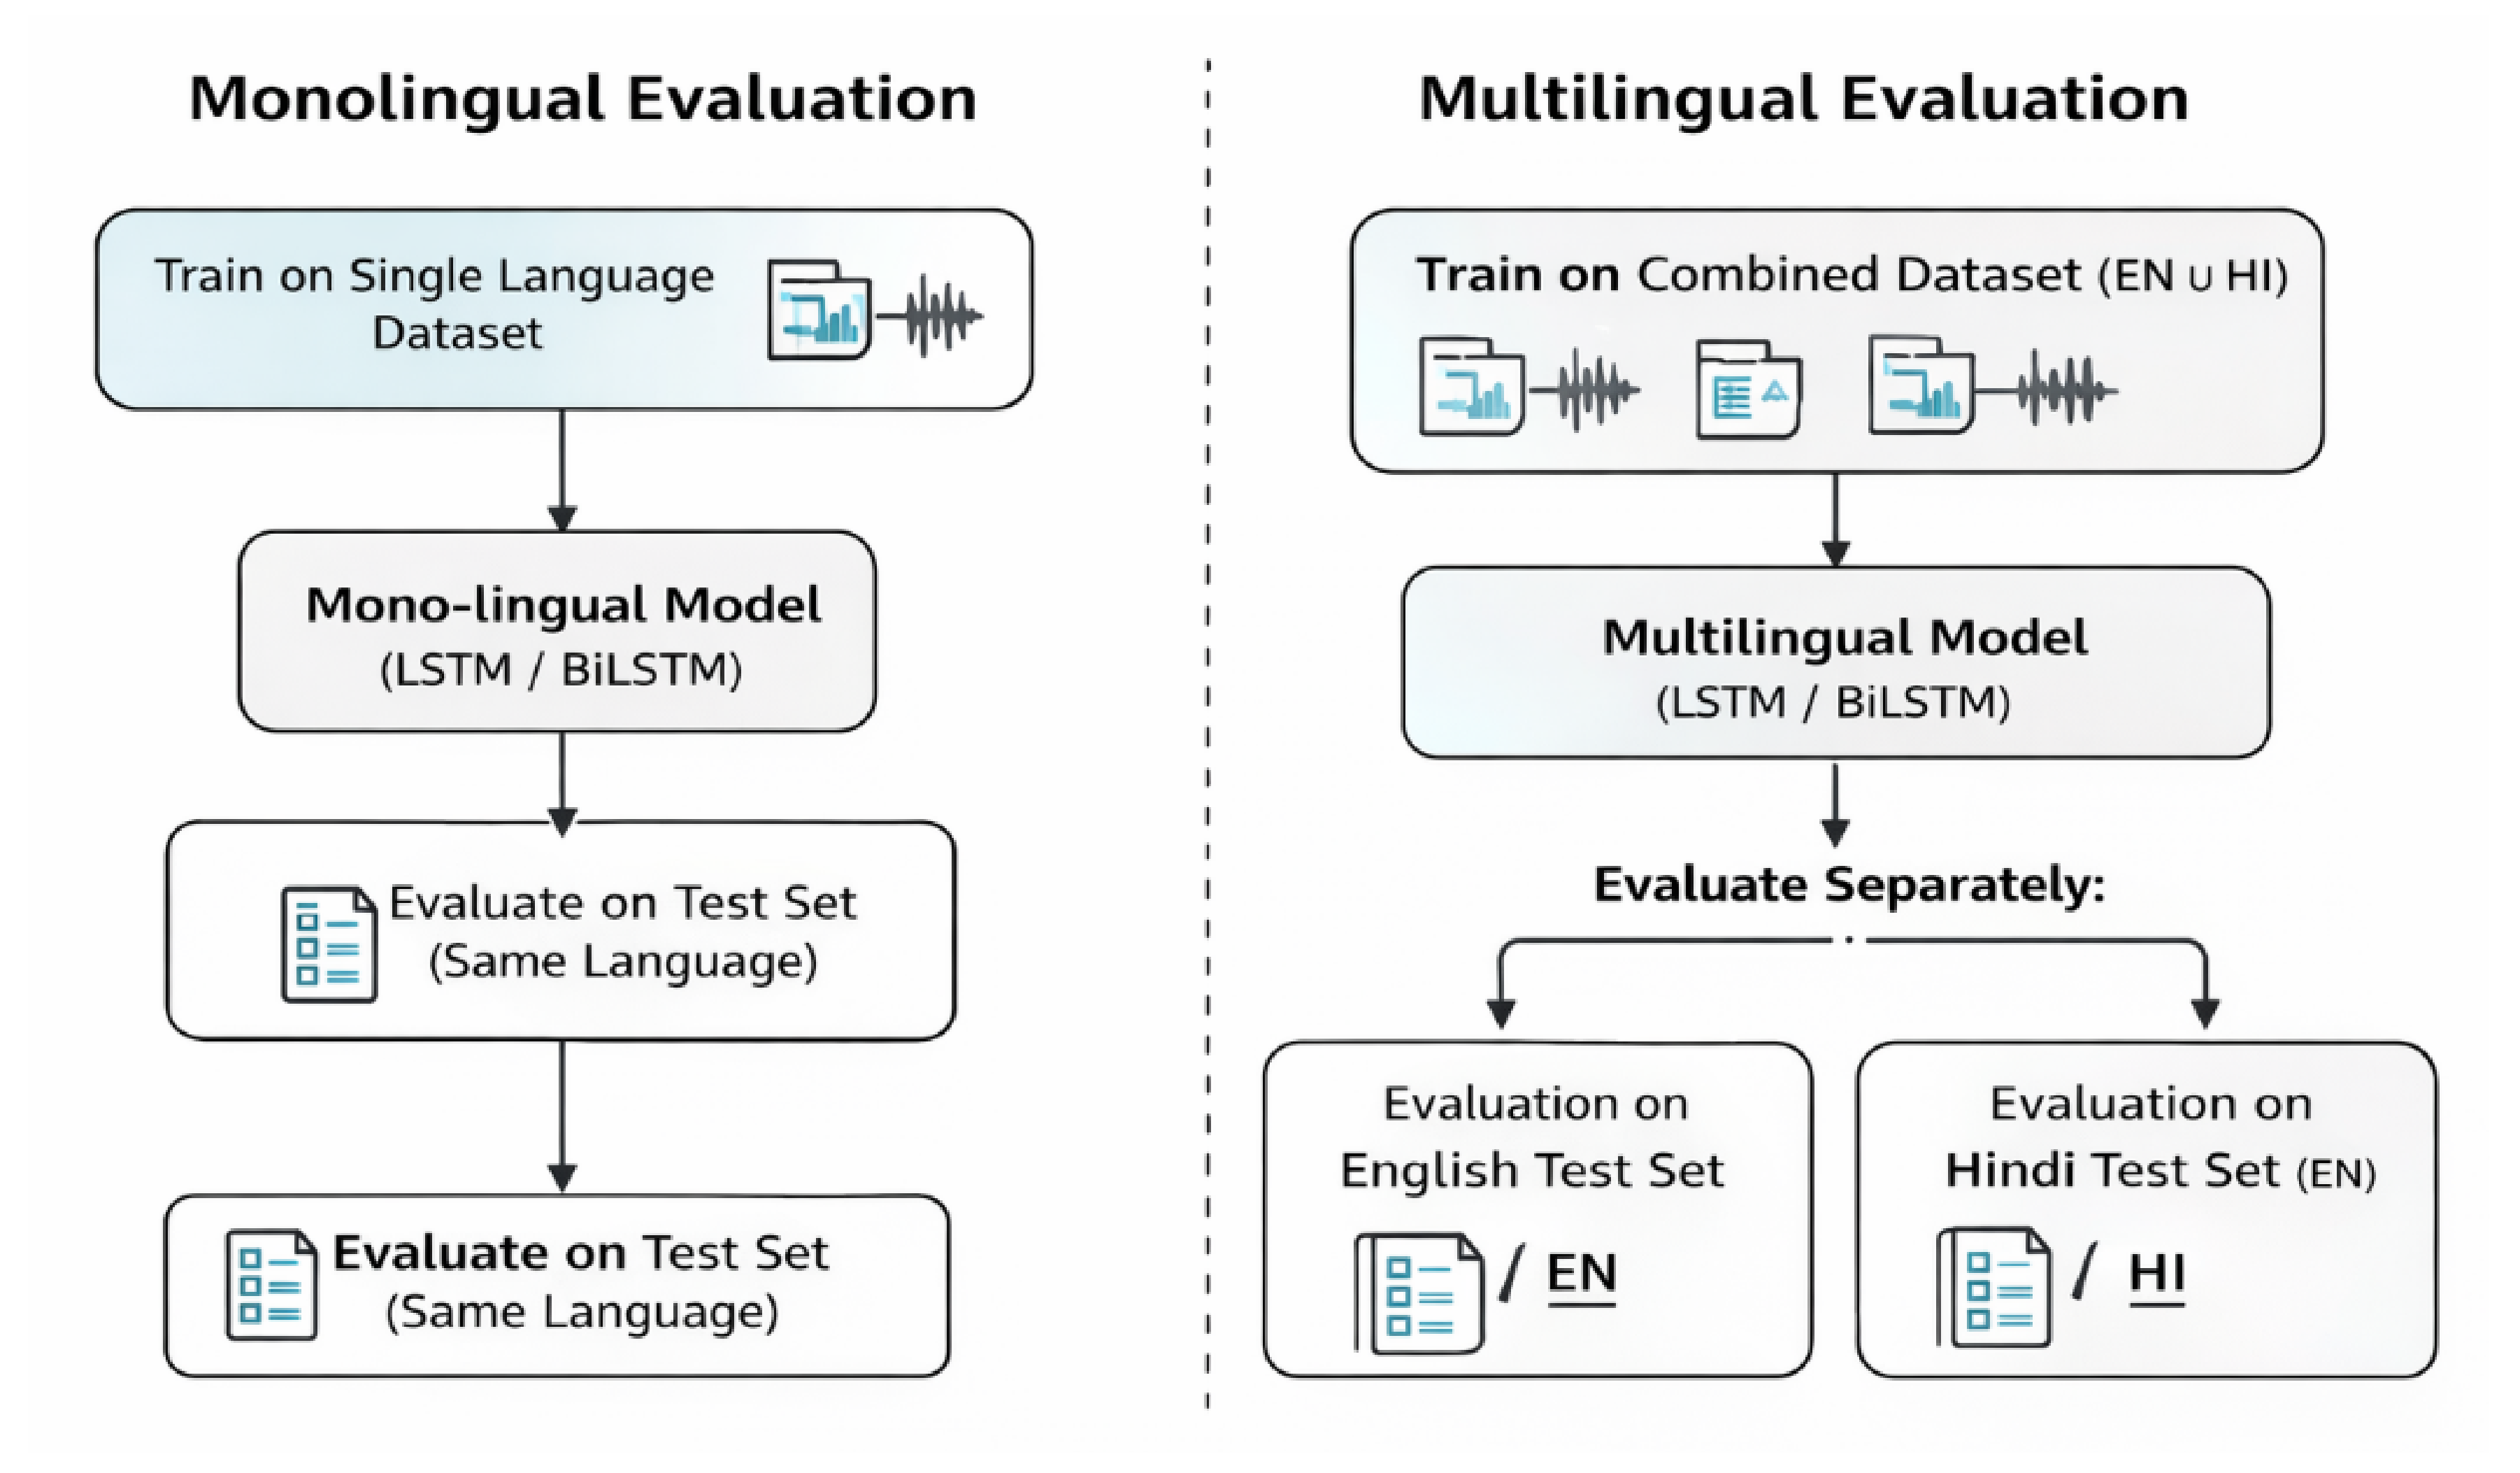
\includegraphics[width=\linewidth]
{images/figure_3.pdf}
\caption{Mono-lingual and Multi-lingual Evolution}
\label{fig:3}
\end{minipage}

\end{figure}


% In preamble
 % If using pdfLaTeX

% In body
\begin{figure}[htbp]
\centering
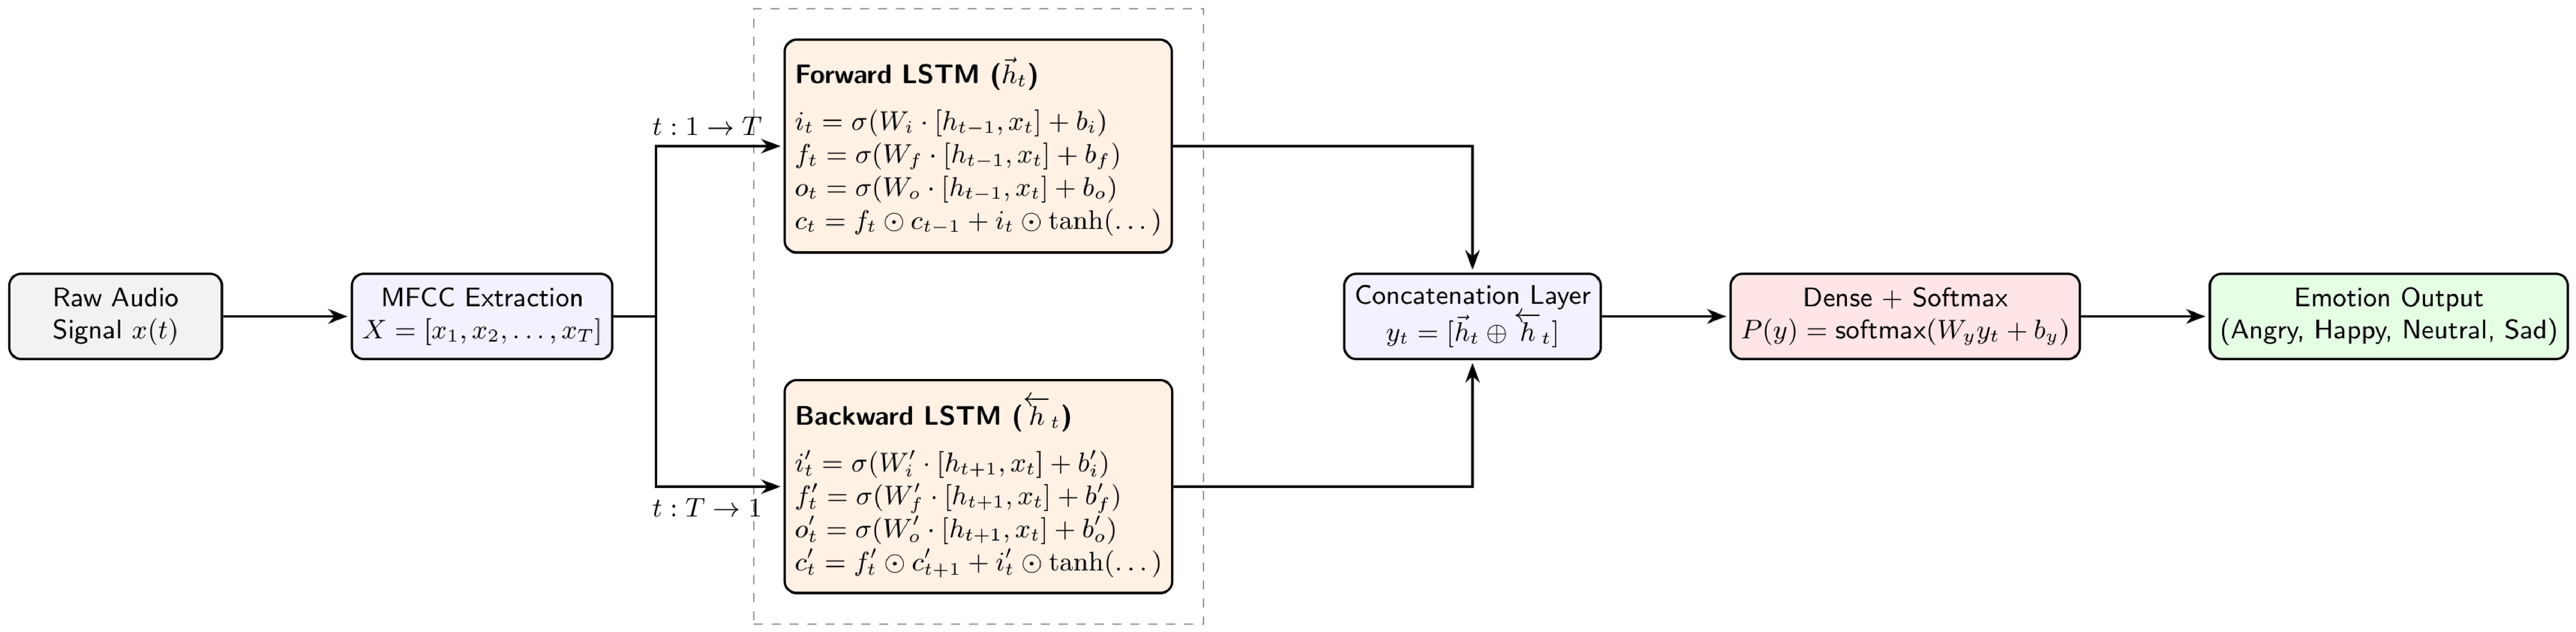
\includegraphics[width=\columnwidth]{images/diagram_cropped-eps-converted-to.pdf}
\caption{Diagram Emotion Classification Baseline model.}
\label{fig:proposed_framework}
\end{figure}

%\subsection{Algorithm for multilingual training and evaluation}
\begin{algorithm}[h]
\caption{Algorithm $\Gamma$: Multilingual MFCC-SER training and evaluation}
\label{alg:gamma}
\begin{algorithmic}[1]
\Require English labeled set $\mathcal{D}^{E}$, Hindi labeled set $\mathcal{D}^{H}$, MFCC extractor $f_{\mathrm{MFCC}}(\cdot)$, duration $\tau$, sample rate $\rho$, MFCC time-steps $T$, folds $\kappa$
\Ensure Mean$\pm$std accuracy on English folds $(\mu^{E},\sigma^{E})$ and Hindi folds $(\mu^{H},\sigma^{H})$
\State \textbf{Preprocess} each waveform $x$ in $\mathcal{D}^{E}\cup\mathcal{D}^{H}$ by padding/truncating to $\tau\cdot\rho$
\State \textbf{Extract} MFCC $M \leftarrow f_{\mathrm{MFCC}}(x)$ and pad/truncate to $T$ frames
\State Form multilingual pool $\mathcal{D}^{M}\leftarrow \mathcal{D}^{E}\cup\mathcal{D}^{H}$
\Statex
\State \textbf{English test view:} split only $\mathcal{D}^{E}$ into $\kappa$ stratified folds
\For{$r=1$ to $\kappa$}
  \State $\mathcal{D}^{E}_{tr}(r),\mathcal{D}^{E}_{te}(r)\leftarrow \text{Split}(\mathcal{D}^{E})$
  \State $\mathcal{D}_{tr}(r)\leftarrow \mathcal{D}^{E}_{tr}(r)\cup \mathcal{D}^{H}$
  \State Train model parameters $\theta_{r}$ on $\mathcal{D}_{tr}(r)$
  \State Evaluate on $\mathcal{D}^{E}_{te}(r)$ to obtain $Acc^{E}_{r}$
\EndFor
\State $\mu^{E}\leftarrow \mathrm{Mean}(\{Acc^{E}_{r}\}),\;\sigma^{E}\leftarrow \mathrm{Std}(\{Acc^{E}_{r}\})$
\Statex
\State \textbf{Hindi test view:} split only $\mathcal{D}^{H}$ into $\kappa$ stratified folds
\For{$r=1$ to $\kappa$}
  \State $\mathcal{D}^{H}_{tr}(r),\mathcal{D}^{H}_{te}(r)\leftarrow \text{Split}(\mathcal{D}^{H})$
  \State $\mathcal{D}_{tr}(r)\leftarrow \mathcal{D}^{H}_{tr}(r)\cup \mathcal{D}^{E}$
  \State Train model parameters $\theta_{r}$ on $\mathcal{D}_{tr}(r)$
  \State Evaluate on $\mathcal{D}^{H}_{te}(r)$ to obtain $Acc^{H}_{r}$
\EndFor
\State $\mu^{H}\leftarrow \mathrm{Mean}(\{Acc^{H}_{r}\}),\;\sigma^{H}\leftarrow \mathrm{Std}(\{Acc^{H}_{r}\})$
\end{algorithmic}
\end{algorithm}


\section{Results and Analysis}
A. Experimental Results
The proposed speech emotion recognition framework was evaluated under monolingual, cross-lingual, multilingual, and Hindi-only experimental settings. The evaluation was carried out using accuracy as the primary metric, along with precision, recall, F1-score, and confusion matrices for detailed analysis. Overall, the results show that model performance varies clearly depending on the training strategy, feature representation, and language setting.
\\
%1) Monolingual Performance
In the monolingual setting, models were trained and tested on speech data from the same language, using RAVDESS for English and IESC for Hindi. For MFCC-based models, both LSTM and Bi-LSTM architectures achieved stable and consistent accuracy across folds. Among them, the Bidirectional LSTM (Bi-LSTM) consistently produced higher accuracy than the unidirectional LSTM. This is because Bi-LSTM processes speech signals in both forward and backward directions, allowing it to capture emotional patterns that appear at different time positions in an utterance. For Hindi-only experiments on the IESC dataset, the MFCC + LSTM model combined with 5-fold stratified cross-validation showed reliable accuracy with low variation across folds. This indicates that the model generalized well to unseen Hindi samples. Emotions such as anger and neutral achieved higher classification accuracy, while sadness and fear showed lower accuracy due to similar acoustic characteristics. Overall, monolingual experiments achieved the highest accuracy levels among all settings, since training and testing data belonged to the same language.

Ravdess Dataset
Table~\ref{tab:ravdess_lstm_mono_eng} presents the classification performance of the MFCC + LSTM model evaluated on the RAVDESS dataset under a mono-lingual setting (Train-ENG, Test-ENG). The model achieved an overall accuracy of 79\%, with highest F1-score observed for Class 4 (0.87), while Class 3 showed relatively lower performance (0.63), indicating potential inter-class confusion. The confusion matrix (Fig. ~\ref{fig:1}) also shows why class 0 has highest recall and class 3 has minimum recall value.

\begin{table}[!htbp]
\caption{Classification Report of RAVDESS Dataset LSTM in Mono-lingual Approach (Train-ENG, Test-ENG)}
\centering
\begin{tabular}{ccccc}
\toprule
\textbf{Class} & \textbf{Precision} & \textbf{Recall} & \textbf{F1-score} & \textbf{Support} \\
\midrule
0 & 0.73 & 0.93 & 0.82 & 153 \\
1 & 0.80 & 0.78 & 0.79 & 153 \\
2 & 0.84 & 0.77 & 0.80 & 154 \\
3 & 0.63 & 0.64 & 0.63 & 154 \\
4 & 0.89 & 0.85 & 0.87 & 154 \\
5 & 0.84 & 0.64 & 0.73 & 153 \\
6 & 0.79 & 0.79 & 0.79 & 154 \\
7 & 0.81 & 0.90 & 0.85 & 154 \\
\midrule
\textbf{Accuracy} &  &  & \textbf{0.79} & \textbf{1229} \\
\bottomrule
\end{tabular}
\label{tab:ravdess_lstm_mono_eng}
\end{table}

\begin{figure}[t]
\centering

\begin{minipage}{0.48\textwidth}
\centering
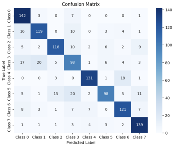
\includegraphics[width=\linewidth]
{images/figure_1.pdf}
\caption{Confusion matrix of RAVDESS Dataset LSTM in Mono-lingual Approach (Train-ENG, Test-ENG).}
\label{fig:1}
\end{minipage}
\hfill
\begin{minipage}{0.48\textwidth}
\centering
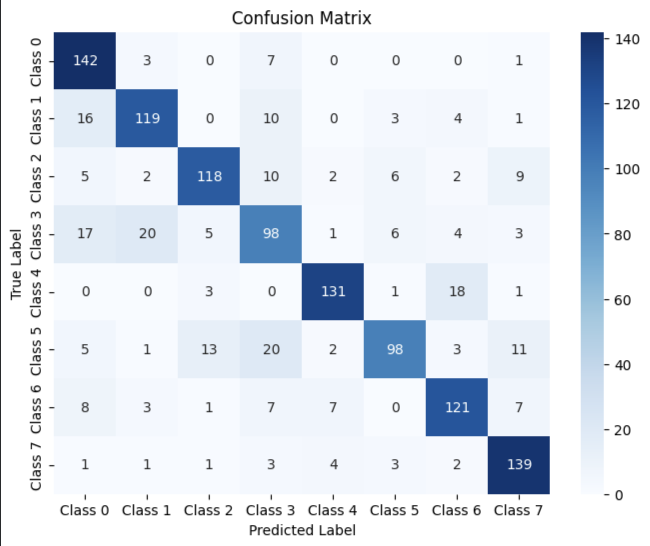
\includegraphics[width=\linewidth]
{images/figure_2.pdf}
\caption{Confusion matrix of RAVDESS Dataset Bi-LSTM in Mono-lingual Approach (Train-ENG, Test-ENG).}
\label{fig:2}
\end{minipage}

\end{figure}


Table~\ref{tab:ravdess_bilstm_mono_eng} presents the classification performance of the MFCC+Bi-LSTM model evaluated on the RAVDESS dataset under a mono-lingual setting (Train-ENG, Test-ENG). The model achieved an overall accuracy of 80\%, with the highest F1-scores observed for Classes 4 and 7 (0.86). Compared to the standard LSTM model, the Bi-LSTM architecture demonstrates improved contextual learning capability, particularly in recall performance for Classes 6 and 7. The confusion matrix (Fig. ~\ref{fig:2}) also shows why class 0 has highest recall and class 3 has minimum recall value.

\begin{table}[!htbp]
\caption{Classification Report of RAVDESS Dataset Bi-LSTM in Mono-lingual Approach (Train-ENG, Test-ENG)}
\centering
\begin{tabular}{ccccc}
\toprule
\textbf{Class} & \textbf{Precision} & \textbf{Recall} & \textbf{F1-score} & \textbf{Support} \\
\midrule
0 & 0.78 & 0.93 & 0.85 & 153 \\
1 & 0.80 & 0.86 & 0.83 & 153 \\
2 & 0.80 & 0.68 & 0.73 & 154 \\
3 & 0.72 & 0.59 & 0.65 & 154 \\
4 & 0.90 & 0.83 & 0.86 & 154 \\
5 & 0.76 & 0.72 & 0.74 & 153 \\
6 & 0.78 & 0.88 & 0.82 & 154 \\
7 & 0.83 & 0.89 & 0.86 & 154 \\
\midrule
\textbf{Accuracy} &  &  & \textbf{0.80} & \textbf{1229} \\
\bottomrule
\end{tabular}
\label{tab:ravdess_bilstm_mono_eng}
\end{table}

Hindi Dataset Table~\ref{tab:iedc_hindi_lstm_mono} presents the performance of the LSTM model on the IEDC Hindi dataset under a mono-lingual setting (Train-Hindi, Test-Hindi). The model achieved an overall accuracy of 90\%, with strong F1-scores across all emotion classes. The highest precision was observed for the Happy class (0.95), while Sad exhibited the highest recall (0.93), indicating effective emotional discrimination in the Hindi speech domain.

\begin{table}[!htbp]
\caption{Classification Report of IESC Hindi Dataset LSTM in Mono-lingual Approach (Train-Hindi, Test-Hindi)}
\centering
\begin{tabular}{ccccc}
\toprule
\textbf{Emotion} & \textbf{Precision} & \textbf{Recall} & \textbf{F1-score} & \textbf{Support} \\
\midrule
Anger & 0.90 & 0.92 & 0.91 & 120 \\
Sad & 0.84 & 0.93 & 0.88 & 120 \\
Happy & 0.95 & 0.87 & 0.90 & 120 \\
Fear & 0.94 & 0.89 & 0.91 & 120 \\
\midrule
\textbf{Accuracy} &  &  & \textbf{0.90} & \textbf{480} \\
\bottomrule
\end{tabular}
\label{tab:iedc_hindi_lstm_mono}
\end{table}


\begin{figure}[t]
\centering

\begin{minipage}{0.48\textwidth}
\centering
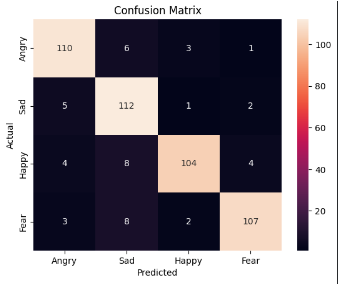
\includegraphics[width=\linewidth]
{images/figure_8.pdf}
\caption{Confusion Matrix of IESC Hindi Dataset LSTM in Mono-lingual Approach (Train-Hindi, Test-Hindi).}
\label{fig:8}
\end{minipage}
\hfill
\begin{minipage}{0.48\textwidth}
\centering
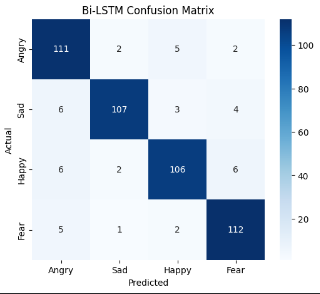
\includegraphics[width=\linewidth]
{images/figure_6.pdf}
\caption{Confusion Matrix of IESC Hindi Dataset LSTM in Mono-lingual Approach (Train-Hindi, Test-Hindi).}
\label{fig:6}
\end{minipage}

\end{figure}

\begin{table}[!htbp]
\caption{Classification Report of IESC Hindi Dataset Bi-LSTM in Mono-lingual Approach (Train-Hindi, Test-Hindi)}
\centering
\begin{tabular}{ccccc}
\toprule
\textbf{Emotion} & \textbf{Precision} & \textbf{Recall} & \textbf{F1-score} & \textbf{Support} \\
\midrule
Anger & 0.87 & 0.93 & 0.90 & 120 \\
Sad & 0.96 & 0.89 & 0.92 & 120 \\
Happy & 0.91 & 0.88 & 0.90 & 120 \\
Fear & 0.90 & 0.93 & 0.92 & 120 \\
\midrule
\textbf{Accuracy} &  &  & \textbf{0.91} & \textbf{480} \\
\bottomrule
\end{tabular}
\label{tab:iedc_hindi_bilstm_mono}
\end{table}
Table~\ref{tab:iedc_hindi_bilstm_mono} presents the performance of the MFCC+Bi-LSTM model on the IEDC Hindi dataset under a mono-lingual setting (Train-Hindi, Test-Hindi). The model achieved an overall accuracy of 91\%, with the highest F1-scores observed for the Sad and Fear classes (0.92), demonstrating improved contextual feature learning compared to the standard LSTM model. Fig. ~\ref{fig:8} represent the confusion matrix of IESC Hindi Dataset LSTM in Mono-lingual Approach (Train-Hindi, Test-Hindi). I the fig. ~\ref{fig:6} shows the Bi-LSTM confusion matrix.

%3) Multilingual Training Results

In the multilingual setting, models were trained on combined Hindi and English speech data and evaluated on both languages. Multilingual training resulted in higher and more stable accuracy compared to cross-lingual training alone. Exposure to speech from multiple languages during training allowed the models to learn shared emotional patterns, reducing language bias. The Bi-LSTM model with MFCC features achieved better average accuracy than the unidirectional LSTM. These results show that multilingual training improves robustness and reduces accuracy variation, making the system more suitable for real-world multilingual applications.
Table \ref{tab:multilingual_results} presents the performance of LSTM and Bi-LSTM models under multi-lingual training condition. It is observed that Bi-LSTM model obtained higher test accuracy and macro-F1 score compared to LSTM for English evaluation. However, there is a slightly decrease in performance observed for Hindi evaluation.

%4) Hindi IESC Dataset with Stratified K-Fold Evaluation

% ---- Added: Hindi IESC Stratified K-Fold table + confusion matrix + classification report ----
\begin{table}[!htbp]
\caption{Performance Comparison under Multilingual Training (Train: English + Hindi, Test: English and Hindi)}
\centering
\begin{tabular}{p{1.8cm} p{2cm} p{3.2cm} p{3cm} p{2cm}}
\hline
\textbf{Test Language} & \textbf{Model} & \textbf{Train Accuracy (Mean $\pm$ Std)} & \textbf{Test Accuracy (Mean $\pm$ Std)} & \textbf{Macro-F1} \\
\hline
English & MFCC+ LSTM & 0.9304 $\pm$ 0.0326 & 0.7992 $\pm$ 0.0293 & 0.7861 \\
English & MFCC+ Bi-LSTM & 0.9872 $\pm$ 0.0093 & 0.8472 $\pm$ 0.0266 & 0.8400 \\
\hline
Hindi & MFCC+ LSTM & $0.8774 $\pm $ 0.0058$ \quad & 0.8063 $\pm$ 0.0579 & 0.8054 \\
Hindi & MFCC+ Bi-LSTM & $0.8795 \pm 0.0148$ & 0.7842 $\pm$ 0.0859 & 0.7832 \\
\hline
\end{tabular}
\label{tab:multilingual_results}
\end{table}


% (Could not reliably detect the Hindi IESC confusion/classification figures from the DOCX order.)

Table~\ref{tab:multilingual_lstm_test_eng} presents the performance of the MFCC+LSTM model trained on a multi-lingual dataset and evaluated on English speech samples. The overall accuracy achieved is 79\%, with the highest F1-score observed for the Anger class (0.88). The Neutral class exhibits comparatively lower performance, indicating potential cross-lingual variability in neutral speech characteristics.

\begin{table}[!htbp]
\caption{Classification Report of Multi-lingual Emotion Dataset using LSTM in Multi-lingual Approach (Train-Multi-lingual, Test-Eng)}
\centering
\begin{tabular}{ccccc}
\toprule
\textbf{Emotion} & \textbf{Precision} & \textbf{Recall} & \textbf{F1-score} & \textbf{Support} \\
\midrule
Anger   & 0.90 & 0.86 & 0.88 & 768 \\
Sad     & 0.77 & 0.76 & 0.77 & 768 \\
Happy   & 0.76 & 0.79 & 0.78 & 768 \\
Fear    & 0.83 & 0.82 & 0.83 & 768 \\
Neutral & 0.65 & 0.66 & 0.66 & 384 \\
\midrule
\textbf{Accuracy} &  &  & \textbf{0.79} & \textbf{3456} \\
\bottomrule
\end{tabular}
\label{tab:multilingual_lstm_test_eng}
\end{table}


\begin{figure}[t]
\centering

\begin{minipage}{0.48\textwidth}
\centering
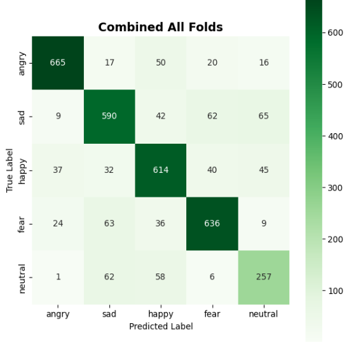
\includegraphics[width=\linewidth]
{images/confmat_multilingual_lstm.png}
\caption{Confusion Matrix of MFCC + LSTM Model (Combined All Folds).}
\label{fig:confmat_multilingual_lstm}
\end{minipage}
\hfill
\begin{minipage}{0.48\textwidth}
\centering
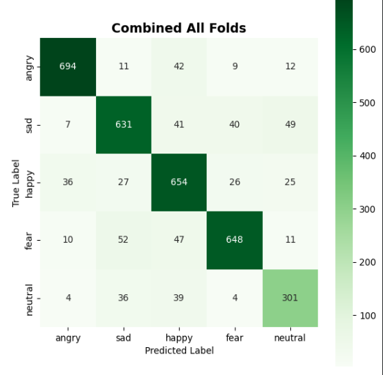
\includegraphics[width=\linewidth]
{images/confmat_multilingual_Bilstm.png}
\caption{Confusion Matrix of MFCC + Bi-LSTM Model (Combined All Folds).}
\label{fig:confmat_multilingual_Bilstm.png}
\end{minipage}

\end{figure}


\begin{table}[!htbp]
\caption{Classification Report of Multi-lingual Emotion Dataset using Bi-LSTM in Multi-lingual Approach (Train-Multi-lingual, Test-Eng)}
\centering
\begin{tabular}{ccccc}
\toprule
\textbf{Emotion} & \textbf{Precision} & \textbf{Recall} & \textbf{F1-score} & \textbf{Support} \\
\midrule
Anger   & 0.92 & 0.90 & 0.91 & 768 \\
Sad     & 0.83 & 0.82 & 0.82 & 768 \\
Happy   & 0.79 & 0.85 & 0.82 & 768 \\
Fear    & 0.89 & 0.84 & 0.86 & 768 \\
Neutral & 0.75 & 0.78 & 0.76 & 384 \\
\midrule
\textbf{Accuracy} &  &  & \textbf{0.84} & \textbf{3456} \\
\bottomrule
\end{tabular}
\label{tab:multilingual_bilstm_test_hindi}
\end{table}
Table~\ref{tab:multilingual_bilstm_test_hindi} presents the performance of the MFCC+Bi-LSTM model trained on multi-lingual data and evaluated on Hindi speech samples. The model achieved an overall accuracy of 84\%, demonstrating improved contextual representation compared to the standard LSTM model, particularly in the Anger (F1 = 0.91) and Fear (F1 = 0.86) classes. Fig. ~\ref{fig:confmat_multilingual_lstm} represent the Confusion Matrix of MFCC + LSTM Model (Combined All Folds).
The Hindi IESC dataset was evaluated separately using 5-fold stratified cross-validation. The LSTM model with MFCC features produced consistent accuracy across all folds, indicating reliable learning behavior. Stratified K-fold validation ensured that each fold contained a balanced distribution of emotion classes, which reduced bias and produced a more accurate estimate of real-world performance. The average accuracy across folds remained stable, with only minor fluctuations. Confusion matrix analysis showed that anger and happiness were classified with higher accuracy, while sadness and fear were more frequently confused due to acoustic similarity. These findings are consistent with existing speech emotion recognition studies. Fig.~\ref{fig:confmat_multilingual_Bilstm.png} shows the Confusion Matrix of MFCC + Bi-LSTM Model (Combined All Folds).
\section{Discussion}
The comparison between LSTM and Bi-LSTM based models clearly highlights that the choice of architecture has a strong impact on accuracy. LSTM models achieved a good baseline accuracy. Bi-LSTM models consistently improved accuracy by capturing both past and future speech contexts. This shows that context-aware and pretrained models are better suited for emotion recognition across languages. MFCC features provided reasonable accuracy in monolingual and multilingual settings and performed well when combined with Bi-LSTM architectures. However, MFCC-based models showed larger accuracy drops in cross-lingual experiments. The achieved accuracy levels across monolingual, and multilingual settings show that speech emotion recognition systems can generalize reasonably well across languages. Such systems can be useful in emotion-aware human–computer interaction, call-centre analysis, and mental health support tools, especially in multilingual and low-resource environments. The system is not intended for diagnosis, but its ability to detect broad emotional states can help provide early emotional awareness.

% 4) Limitations and Future Scope

% Despite good accuracy, several limitations remain. The datasets mainly contain acted emotional speech, which may differ from real-world spontaneous emotions. Cross-lingual accuracy is also affected by cultural and linguistic differences. Deep models such as Bi-LSTM require high computational resources, which may limit deployment on low-power devices. Future work can focus on lighter models, model compression, and multimodal approaches to further improve accuracy and usability. The experimental results confirm that accuracy is highest in monolingual settings, followed by multilingual, settings. BI-LSTM models outperform LSTM models in terms of accuracy across all experiments. Stratified K-Fold validation provides reliable and stable accuracy estimates. Speech-based emotion recognition shows strong potential for scalable and multilingual emotion-aware systems.

% In the multilingual training setup (training on pooled English + Hindi data and evaluating on the Hindi (IESC) test set), both MFCC-based recurrent models demonstrate strong generalization, indicating that the learned temporal emotion cues captured via MFCC sequences transfer reasonably well across mixed-language training distributions. The overall trend shows that incorporating multilingual data helps the model learn more robust acoustic patterns (e.g., energy contours, spectral dynamics, and prosodic correlates embedded in MFCC trajectories), which is beneficial when the target test language is Hindi.

% From the class-wise behavior (radar chart), angry remains the most consistently separable emotion, with the highest F1 for both models. This is expected because anger typically manifests with stronger intensity, higher energy, and sharper spectral transitions—traits that MFCCs capture effectively. Neutral also achieves relatively high F1, likely due to its stable prosody and reduced variability compared to expressive emotions.

% Performance drops are more visible for fear and happy, which often overlap acoustically (pitch variability, voice quality differences, and speaking rate changes) and are more sensitive to speaker/style variation. In multilingual pooling, such classes can suffer from domain mismatch (recording conditions, speaker demographics, elicitation style) and language-dependent prosody differences, causing inter-class boundary blur even with the same label set.

% Comparing architectures, the Bi-LSTM is generally expected to help when emotion cues depend on both past and future context within an utterance. However, the Hindi-test class-wise results show that LSTM achieves higher F1 for most classes, while Bi-LSTM is only marginally better (or comparable) for fear. This indicates that (i) bidirectional context may not always translate into better generalization under domain/language shifts, and (ii) Bi-LSTM may be more sensitive to training noise or distribution mismatch when pooling multilingual corpora. In practice, the better model may depend on the exact split, speaker composition, and regularization settings; hence, reporting mean±std over folds (as you are doing) is essential for stable IEEE-style claims.

\section{Conclusion}
This study presented a structured bilingual benchmarking of MFCC-based recurrent models for speech emotion recognition under monolingual and multilingual training settings. Experimental results demonstrate that Bi-LSTM architectures consistently outperform unidirectional LSTM by effectively capturing contextual dependencies in speech signals. Monolingual experiments achieved higher peak accuracy, while multilingual pooling enhanced robustness and reduced performance variability across folds.Despite promising results, cross-language variability and acoustic overlap between certain emotions (e.g., fear and sadness) continue to challenge generalization. The reliance on acted datasets further limits real-world deployment readiness.Rather than proposing a novel architecture, this work contributes a controlled empirical evaluation emphasizing fold-wise stability, per-class diagnostics, and reproducible bilingual experimentation. Future research will explore domain-robust training, lightweight attention mechanisms, and multimodal fusion strategies to improve cross-lingual emotional transfer.
\clearpage
\bibliographystyle{splncs04}

\begin{thebibliography}{99}

\bibitem{Yadav2026Misogyny}
Yadav, S., Kaushik, A., \& Daid, K. M. (2026).
An under-explored application for explainable multimodal misogyny detection in code-mixed Hindi-English.
\textit{arXiv preprint arXiv:2601.08457}.

\bibitem{Bhagath2026MultilingualCNN}
Bhagath, P., Prasanna, K. V. L., Sravya, B., \& Mouli, T. (2026).
Multi-lingual spoken language modeling via CNNs for low-resource languages.
\textit{IAENG International Journal of Applied Mathematics}, 56(1).

\bibitem{Haidar2025SERLSTM}
Haidar, S. W., Chaubey, S. K., Mishra, A. D., Akhtar, M. M., Khan, N. A., \& Usmani, T. A. (2025).
Deep learning driven automated system for speech emotion recognition.
In \textit{Proceedings of the IEEE International Conference on Computing, Communication and Automation (ICCCA)} (pp. 1--6). IEEE.

\bibitem{Xu2021HeadFusion}
Xu, M., Zhang, F., \& Zhang, W. (2021).
Head fusion: Improving the accuracy and robustness of speech emotion recognition on the IEMOCAP and RAVDESS dataset.
\textit{IEEE Access}, 9, 74539--74549.

\bibitem{Li2026AAMICASA}
Li, J., Liang, C., Liu, Z., \& Ge, F. (2026).
Speech emotion recognition based on the adaptive acoustic enhancement and refined attention mechanism.
\textit{Computers, Materials \& Continua}, 86(3).

\bibitem{Trigeorgis2016Adieu}
Trigeorgis, G., Ringeval, F., Brueckner, R., Marchi, E., Nicolaou, M. A., Schuller, B., \& Zafeiriou, S. (2016).
End-to-end speech emotion recognition using a deep convolutional recurrent network.
In \textit{Proceedings of IEEE ICASSP} (pp. 5200--5204). IEEE.

\bibitem{Baevski2020Wav2Vec2}
Baevski, A., Zhou, Y., Mohamed, A., \& Auli, M. (2020).
Wav2Vec 2.0: A framework for self-supervised learning of speech representations.
\textit{Advances in Neural Information Processing Systems}, 33, 12449--12460.

\bibitem{Busso2008IEMOCAP}
Busso, C., Bulut, M., Lee, C. C., Kazemzadeh, A., Mower, E., Kim, S., Chang, J. N., Lee, S., \& Narayanan, S. S. (2008).
IEMOCAP: Interactive emotional dyadic motion capture database.
\textit{Language Resources and Evaluation}, 42(4), 335--359.

\bibitem{Chen2022WavLM}
Chen, S., Wang, C., Chen, Z., Wu, Y., Liu, S., Chen, Z., Li, J., Kanda, N., Yoshioka, T., Xiao, X., et al. (2022).
WavLM: Large-scale self-supervised pre-training for full stack speech processing.
\textit{IEEE Journal of Selected Topics in Signal Processing}, 16(6), 1505--1518.

\bibitem{ElAyadi2011Survey}
El Ayadi, M., Kamel, M. S., \& Karray, F. (2011).
Survey on speech emotion recognition: Features, classification schemes, and databases.
\textit{Pattern Recognition}, 44(3), 572--587.

\bibitem{Eyben2010OpenSMILE}
Eyben, F., W{\"o}llmer, M., \& Schuller, B. (2010).
openSMILE: The Munich versatile and fast open-source audio feature extractor.
In \textit{Proceedings of the ACM International Conference on Multimedia} (pp. 1459--1462).

\bibitem{Graves2005BiLSTM}
Graves, A., \& Schmidhuber, J. (2005).
Framewise phoneme classification with bidirectional LSTM and other neural network architectures.
\textit{Neural Networks}, 18(5-6), 602--610.

\bibitem{Hochreiter1997LSTM}
Hochreiter, S., \& Schmidhuber, J. (1997).
Long short-term memory.
\textit{Neural Computation}, 9(8), 1735--1780.

\bibitem{Hsu2021HuBERT}
Hsu, W.-N., Bolte, B., Tsai, Y.-H. H., Lakhotia, K., Salakhutdinov, R., \& Mohamed, A. (2021).
HuBERT: Self-supervised speech representation learning by masked prediction of hidden units.
\textit{IEEE/ACM Transactions on Audio, Speech, and Language Processing}, 29, 3451--3460.

\bibitem{Livingstone2018RAVDESS}
Livingstone, S. R., \& Russo, F. A. (2018).
The Ryerson audio-visual database of emotional speech and song (RAVDESS): A dynamic, multimodal set of facial and vocal expressions in North American English.
\textit{PLOS ONE}, 13(5), e0196391.

\bibitem{Schuller2011Challenge}
Schuller, B., Batliner, A., Steidl, S., \& Seppi, D. (2011).
Recognising realistic emotions and affect in speech: State of the art and lessons learnt from the first challenge.
\textit{Speech Communication}, 53(9-10), 1062--1087.

\bibitem{bhattacharya2022deep}
Bhattacharya, S., Borah, S., Mishra, B. K., \& Das, N. (2022).
Deep analysis for speech emotion recognition.
In \textit{Proceedings of ICCSEA} (pp. 1--6). IEEE.

\bibitem{Bhattacharya2024CrossLingual}
Bhattacharya, S., Mishra, B. K., Borah, S., Das, N., \& Dey, N. (2024).
Cross-lingual deep learning model for gender-based emotion detection.
\textit{Multimedia Tools and Applications}, 83(9), 25969--26007.

\bibitem{Bhattacharya2024MultimodalKFold}
Bhattacharya, S., Borah, S., \& Mishra, B. K. (2024).
Deep multimodal k-fold model for emotion and sentiment analysis in figurative language.
\textit{SSRN Electronic Journal}.


\end{thebibliography}

\end{document}

